\chapter{Results and Discussion}
\label{ch:results}

All figures were read from the running stack, started from a fresh clone
with \code{make up}; the DAG reconciled four simulated days unattended.

\section{The Consistency Argument}
\label{sec:consistency}

The speed layer uses a 10-simulated-minute watermark while the simulator
injects lateness of up to 20 minutes, so the layers are \emph{built} to
disagree (Figure~\ref{fig:consistency}); a regression test stops anyone
widening the watermark to hide this.

\begin{figure}[htbp]
\centering
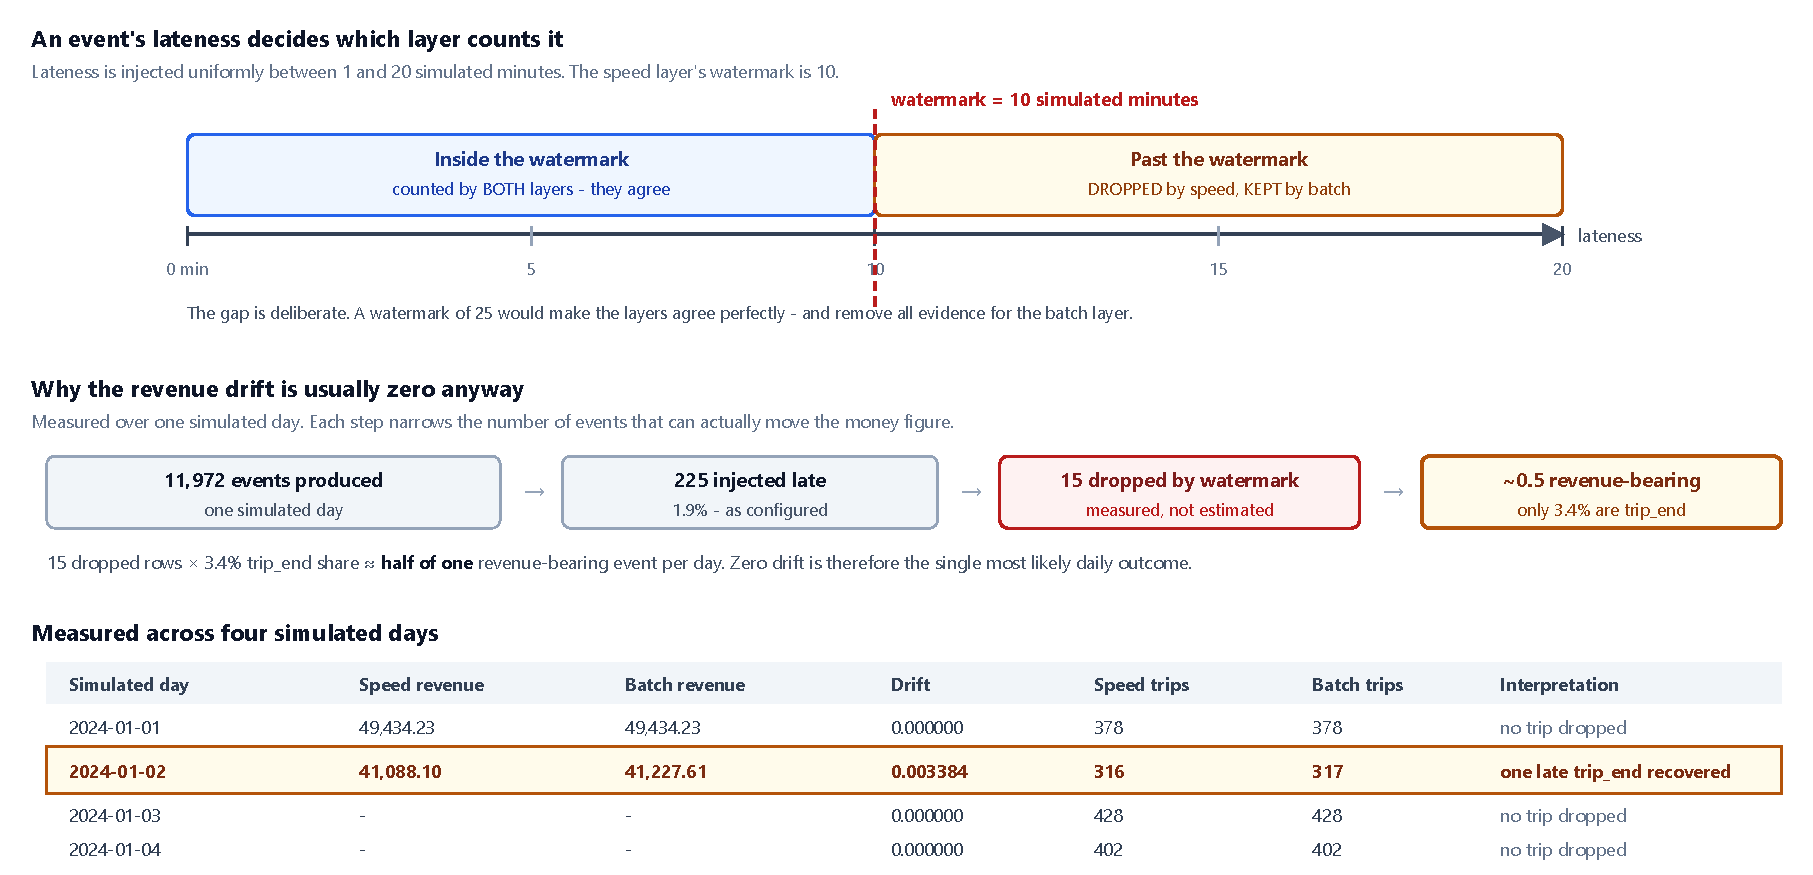
\includegraphics[width=0.9\textwidth]{figures/fig2-consistency.pdf}
\caption[Why the two layers disagree]{Why the two layers disagree: an
event's lateness decides which layer counts it.}
\label{fig:consistency}
\end{figure}

\begin{table}[htbp]
\centering
\caption{Reconciliation outcomes over four simulated days.}
\label{tab:four-days}
\begin{tabularx}{\textwidth}{@{}lRRRRR@{}}
\toprule
\textbf{Simulated day} & \textbf{Fleet margin} & \textbf{Unprof.} &
\textbf{Becoming unprof.} & \textbf{Dist. mismatch} &
\textbf{Revenue drift}\\
\midrule
2024-01-01 (partial) & 42.8\% & 6 & 0 & 2 & 0.000000\\
2024-01-02           & 38.3\% & 4 & 0 & 21 & \textbf{0.003384}\\
2024-01-03           & 45.8\% & 3 & 6 & 6 & 0.000000\\
2024-01-04           & 47.7\% & 4 & 7 & 4 & 0.000000\\
\bottomrule
\end{tabularx}
\end{table}

On 2024-01-02 the speed layer counted 316 trips against the batch
layer's 317: one late \code{trip\_end} dropped by the watermark and
recovered by the batch layer. Drift is usually zero because, per day, the
watermark drops about 15 rows and only 3.4\% of events are
\code{trip\_end}, so the expected number of lost revenue events is
$15 \times 0.034 \approx 0.5$. \code{fleet\_late\_rows\_dropped\_total}
therefore shows the \emph{mechanism} (reliably non-zero) and
\code{fleet\_speed\_batch\_drift\_ratio} its \emph{financial weight}
(usually zero). The case for batch-computed money is not that the speed
layer is badly wrong, but that its error is unbounded in principle, and
no watermark can absorb a correction arriving weeks later.

\section{Recomputation Demonstrated}
\label{sec:recompute}

Dropping a \code{v2} expense file for a reconciled day made it pending
again; the recompute produced \textbf{the same 50 rows with new values}
(net profit 19,770.78 $\rightarrow$ 21,177.99). A forced rerun of
2024-01-03 returned \textbf{bit-identical figures} (net 24,902.95). The
restatement came from one Parquet partition, with no log replay.

\section{Verification}
\label{sec:alerting-results}

\begin{itemize}
  \item 202 unit, PySpark and API tests pass; the smoke test passes 28/28
        checks; all 13 services start healthy from a fresh clone.
  \item 5 of 10 alert rules were observed firing \emph{and} delivered;
        \code{BatchRunFailed} is deliberately inhibited when
        \code{ExpenseFileLate} explains the same failure.
  \item 23 of 23 Grafana panel queries return live data.
  \item Batch task times: \code{compute\_vehicle\_day} 9.44\,s,
        \code{load\_batch\_views} 0.99\,s, all others under 0.5\,s.
\end{itemize}

\section{Discussion}
\label{sec:discussion}

\textbf{Defects found by operating the system.} \label{sec:defects}
Six defects surfaced only at runtime. The most
serious: a Spark worker restart killed the archiver's executor while the
query stayed ``active'', so the \textbf{healthcheck stayed green} while
nothing was archived for 26 minutes (fixed by a progress watchdog).
Others: an odometer checkpoint every 30 real seconds (30 simulated
minutes) that caused false distance mismatches; uncalibrated economics
flagging 35 of 50 vehicles unprofitable; batch gauges exported by every
service, firing a permanent false alert; an expense SLA applied to
corrected \code{v2} files; and two Windows-only start-up bugs.

\textbf{Limitations.} Four days is one run of one configuration, and
day~1 is partial. \code{becoming\_unprofitable} needs three reconciled
days to fire. Batch Spark runs in local mode and Kafka has a single
broker at RF~1. Because simulated time follows the wall clock, downtime
appears in the data as low demand.

\textbf{At production scale.} \label{sec:production}
Kafka would move to three brokers at RF~3 with a
schema registry (keeping the \code{vehicle\_id} key); the lake would use
object storage with a table format such as Iceberg or Delta and
compaction; processing would run on Kubernetes with the archiver
separated from the speed layer; and observability would add log
aggregation, tracing, and SLOs with ratio-based thresholds.
